%!TEX root = ../rapport.tex
%!TEX encoding = UTF-8 Unicode

% Chapitres "Introduction"

% modifié par Francis Valois, Université Laval
% 31/01/2011 - version 1.0 - Création du document

\chapter{Description des cas d'utilisation}
\label{s:utilisation}
Cette section contient un résumé de chacun des différents cas d'utilisation. Elle est divisée en trois parties: soit les cas d'utilisation en lien avec l'usager, ceux en lien avec la station de base et finalement ceux en lien au robot. Le diagramme des cas d'utilisation est présenté à la section \ref{use_cases}.
\section{Cas d'utilisation en lien avec l'usager}
\subsection{Lancer le signal de départ}
À l'aide d'une Graphical user interface ou interface graphique pour utilisateur (GUI) installée sur la station de base, l'utilisateur clique sur un bouton qui lance l'exécution de la séquence (signal de départ transmis au robot pour commencer à effectuer une tâche).
\subsection{Entrer les coordonnées initiales du robot}
Avant d'envoyer le signal de départ au robot, l'utilisateur doit pouvoir entrer les coordonnées de la position de départ du robot par rapport au terrain de jeu sur la station de base.
\section{Cas d'utilisations en lien avec la station de base}
\subsection{Localiser le robot}
À l'aide de la Kinect, la station de base doit être en mesure de trouver la position du robot sur le terrain de jeu.
\subsection{Détecter les obstacles}
Au moyen de la Kinect, la station de base doit détecter la position des deux obstacles disposés entre les deux zones principales du terrain de jeu ainsi que les limites (murs) du terrain.
\subsection{Afficher la solution du sudocube}
La station de base doit afficher une image du sudocube résolu et indiquer à l'écran le chiffre qui se trouve dans la case rouge du cube.
\subsection{Afficher le message de confirmation du lancement de la tâche}
La station doit afficher un message de confirmation du lancement de la tâche pour l'usager lorsque le message de confirmation du robot est reçu.
\subsection{Afficher la trajectoire prévue et réelle du robot}
La trajectoire calculée et transmise par le robot doit être affichée sur l'écran de la station de base. De plus, à l'aide des données transmises par la Kinect, la station doit afficher la trajectoire prévue et la trajectoire réelle du robot.
\subsection{Transmettre les données au robot}
La station doit transmettre au robot, par connexion sans fil, un message indiquant le début de la tâche et la position des obstacles.
\subsection{Recevoir les données provenant du robot}
La station de base doit recevoir, par connexion sans fil, les données provenant du robot comme la trajectoire qu’il prévoit emprunter, le sudocube résolu, le message de confirmation du lancement d'une tâche et le message indiquant la fin d'une tâche.
\subsection{Afficher le message confirmant que la tâche a été accomplie ou échouée}
La station de base doit afficher un message sur l'écran confirmant que la tâche a été accomplie ou un message d'échec si cette dernière a pris plus de 10 minutes pour s'exécuter.
\subsection{Afficher le temps d'exécution de la tâche}
La station de base doit afficher sur l'écran le temps d'exécution de la tâche.
\section{Cas d'utilisation en lien avec le robot}
\subsection{Déterminer le chemin optimal entre un point A et un point B tout en évitant les obstacles}
Avec la configuration et la position des obstacles, le robot doit calculer la trajectoire optimale pour se rendre d'un point à l'autre.
\subsection{Se déplacer d'un point A au point B}
Le robot doit se déplacer sur le terrain de jeu d'un point A vers un point B avec un contrôle automatisé des roues.
\subsection{Indiquer son adresse IP locale pour que la station de base communique avec le robot}
Le robot doit être capable d'indiquer son adresse IP locale à la station de base pour que celle-ci établisse une connexion sans fil entre eux.
\subsection{Extraire les informations d'un sudocube à partir d'une photo}
À l'aide de la caméra embarquée, il doit prendre une photo et extraire le sudocube à partir de l'image obtenue.
\subsection{Résoudre le sudocube et identifier le chiffre dans le carré rouge}
Le robot doit résoudre le sudocube, identifier l'emplacement de la case rouge à l'intérieur de celui-ci et déterminer le chiffre qui s'y trouve.
\subsection{Recevoir les données provenant de la station de base}
Le robot doit recevoir, par connexion sans fil avec la station de base, les messages indiquant le début de la nouvelle tâche, la position des obstacles et sa position.
\subsection{Transmettre les données à la station de base}
Le robot doit transmettre, par connexion sans-fil à la station de base, la trajectoire qu’il prévoit emprunter, le sudocube résolu, le message de confirmation du lancement d'une tâche et le message indiquant la fin d'une tâche.
\subsection{Contrôler une DEL}
Une fois le message de fin transmis et le robot à l'extérieur de l'aire de dessin, ce dernier doit allumer une DEL qui est installée sur le robot.
\subsection{Lancer une nouvelle tâche si la compétition n'est pas terminée}
Si le temps alloué pour la compétition (10 minutes) n'est pas écoulé, le robot doit commencer une nouvelle tâche après avoir terminé la précédente.
\subsection{Se localiser}
Le robot doit déterminer sa position et son orientation en temps réel à l'aide de la webcam et des données reçues de la station de base. De plus, il doit transmettre ces données à la station de base de façon régulière.
\subsection{Décoder la transmission de l'antenne}
Le robot doit se déplacer au-dessus de l'antenne et capter le signal transmis par celle-ci. Il doit ensuite le décoder afin de trouver les paramètres indiquant le sudocube à résoudre ainsi que l'orientation et la taille du chiffre à dessiner dans la zone de dessin.
\subsection{Dessiner le chiffre du carré rouge en suivant les consignes}
Une fois dans l'aire de dessin, le robot doit utiliser un préhenseur afin de poser la mine du crayon sur la table. Il doit ensuite se déplacer de façon à dessiner le chiffre obtenu dans la case rouge du sudocube, tout en suivant les dimensions et le sens exigés. 
\subsection{Afficher des informations sur l'écran LCD}
Les paramètres trouvés lors du décodage du signal de l'antenne doivent être affichés sur un écran LCD installé sur le robot.
\section{Diagramme des cas d'utilisation}
\label{use_cases}
\addtolength{\evensidemargin}{-1in}	
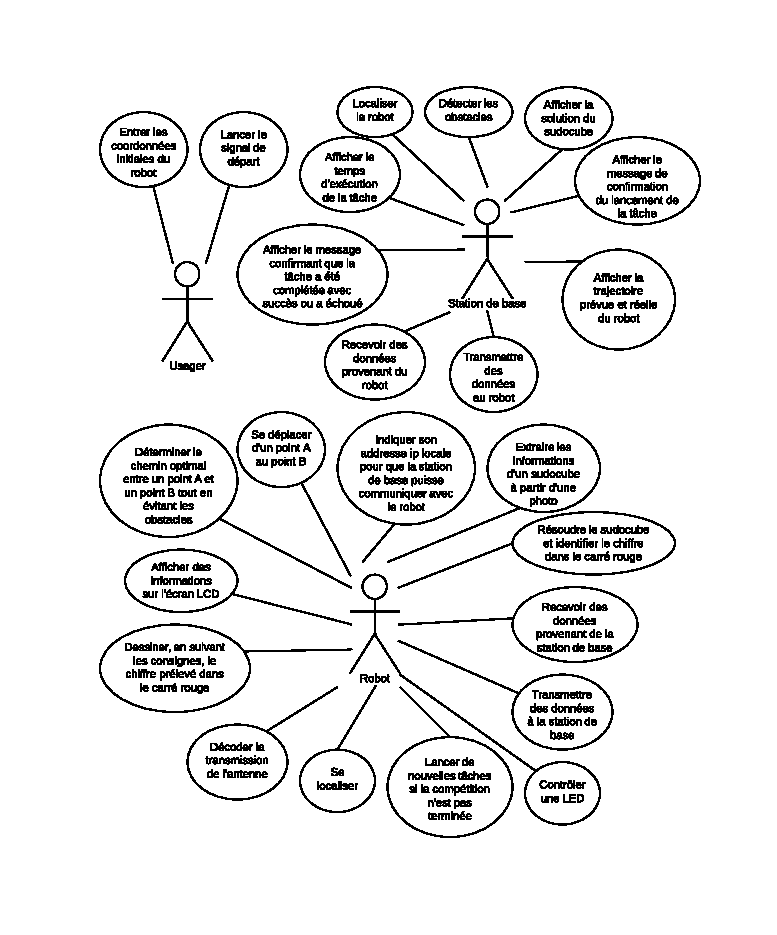
\includepdf[scale= 1]{use_cases_diagram.pdf}